This section describes the basic notions of nonabelian topology which I
formalized and applied to homotopy type theory instead of topological
spaces. The majority of definitions is taken from the book ``Nonabelian
Algebraic Topology'' by Ronald Brown, Philip J. Higgins and Rafael Sivera
\cite{nat}.
The structures used extend classical homotopy theory by considering
\emph{fundamental groupoids} with multiple base points, characterizing the 
interaction between the first and the second homotopy group of a space by 
\emph{crossed modules} as well as \emph{$n$-fold categories} for which we will
only consider the case $n = 2$.

\section{Double Categories}

%TODO difference to higher categories

To make the precise definition of a double category easier, we observe that we
can define a (small) category $C$ by giving a tuple $(ob_C, hom_C, \partial^-,
\partial^+, \epsilon, \circ_C)$ where
\begin{itemize}
\item $ob_C$ is the set of objects,
\item $hom_C$ is a set that contains all morphisms,
\item $\partial^-$ and $\partial^+ : hom_C \to ob_C$
are maps assigning to each morphism $f$ its domain and codomain,
\item $\epsilon : ob_C \to mor_C$ gives the identity morphism at each element
(this implies $\partial^- \circ_C \epsilon = \partial^+ \circ_C \epsilon = \id$),
\item and $\circ_C$
denotes the composition of morphisms as a partial function $hom_C \times hom_C
\to hom_C$, defined for all $(g, f) \in hom_C \times hom_C$ where
$\partial^+(f) = \partial^-(g)$.
\end{itemize}
In line with the geometric interpretation that objects correspond to points while
morphisms correspond to line we will call $\partial^-$ and $\partial^+$
\textbf{boundary} or \textbf{face maps} while $\epsilon$ will often be referred
to as \textbf{degeneracy map}.

\begin{defn}
A \textbf{double category} $D$ is given by the following data:
Three sets $D_0$, $D_1$, and $D_2$, respectively called \textbf{0-, 1- and
2-cells}, together with
maps $\partial^-$, $\partial^+$, $\epsilon$, $\circ_D$,
$\partial^-_1$, $\partial^+_1$, $\epsilon_1$, $\circ_1$,
$\partial^-_2$, $\partial^+_2$, $\epsilon_2$, and $\circ_2$
such that these sets form three categories:
\begin{itemize}
\item A category $(D_0, D_1, \partial^-, \partial^+, \epsilon, \circ_D)$ 
on $D_0$ often called the \textbf{(1-)skeleton} of the double category.
\item A \textbf{vertical category}
$(D_1, D_2, \partial^-_1, \partial^+_1, \epsilon_1, \circ_1)$ and a 
\item \textbf{horizontal category}
$(D_1, D_2, \partial^-_2, \partial^+_2, \epsilon_2, \circ_2)$.
\end{itemize}

The mentioned maps are required to satisfy the following \textbf{cubical
identities}:
\begin{equation} \label{eq:corner-ident}
\begin{aligned}
\partial^- \circ \partial^-_1 &= \partial^- \circ \partial^-_2\text{,} \\
\partial^- \circ \partial^+_1 &= \partial^+ \circ \partial^-_2\text{,} \\
\partial^+ \circ \partial^-_1 &= \partial^- \circ \partial^+_2\text{,} \\
\partial^+ \circ \partial^+_1 &= \partial^+ \circ \partial^+_2\text{,}
\end{aligned}
\end{equation}
\begin{equation} \label{eq:degen-ident}
\begin{aligned}
\partial^-_1 \circ \epsilon_2 &= \epsilon \circ \partial^-\text{,} \\
\partial^+_1 \circ \epsilon_2 &= \epsilon \circ \partial^+\text{,} \\
\partial^-_2 \circ \epsilon_1 &= \epsilon \circ \partial^-\text{,} \\
\partial^+_2 \circ \epsilon_1 &= \epsilon \circ \partial^+\text{, and}
\end{aligned}
\end{equation}
\begin{equation} \label{eq:zero-unique-ident}
\epsilon_1 \circ \epsilon = \epsilon_2 \circ \epsilon \eqqcolon 0\text{.}	 \\
\end{equation}

The boundary and degeneracy maps of the vertical category are
furthermore assumed to be linear %TODO
in the composition of the horizontal category, and vice versa:
\begin{equation} \label{eq:linear-ident}
\begin{aligned}
\partial^-_2(v \circ_1 u) &= \partial^-_2(v) \circ_D \partial^-_2(u)\text{,} \\
\partial^+_2(v \circ_1 u) &= \partial^+_2(v) \circ_D \partial^+_2(u)\text{,} \\
\partial^-_1(v \circ_2 u) &= \partial^-_1(v) \circ_D \partial^-_1(u)\text{,} \\
\partial^+_1(v \circ_2 u) &= \partial^+_1(v) \circ_D \partial^+_1(u)\text{,} \\
\epsilon_2(g \circ_D f) &= \epsilon_2(g) \circ_1 \epsilon_2(f)\text{, and} \\
\epsilon_1(g \circ_D f) &= \epsilon_1(g) \circ_2 \epsilon_1(g)\text{,}
\end{aligned}
\end{equation}
for each $f, g \in D_1$ and $u, v \in D_2$ where the compositions are defined.

As a last condition, the so called \textbf{interchange law} has to be fulfilled:
For each $u, v, w, x \in D_2$,
\begin{equation}
(x \circ_2 w) \circ_1 (v \circ_2 u) = (x \circ_1 v) \circ_2 (w \circ_1 u)
\end{equation}
has to hold if it is well-defined.
\end{defn}

Especially the identities \ref{eq:corner-ident}, \ref{eq:degen-ident} and the
interchange law might seem arbitrary but their intended meaning becomes more clear
when considering the following geometric interpretation of a double category: We
regard $D_0$ as a set of points, $D_1$ as a set of line segments and
the elements in $D_2$ as squares. Then, $\upperf(u)$, $\lowerf(u)$, $\leftf(u)$ and
$\rightf(u)$ correspond to the upper, lower, left and right face of a square $u$.

As seen in figure \ref{fig:corner-ident}, the four identities \ref{eq:corner-ident}
correspond to the well-definedness of the corners of a given square $u \in D_2$.

\begin{figure} \label{fig:corner-ident} \centering
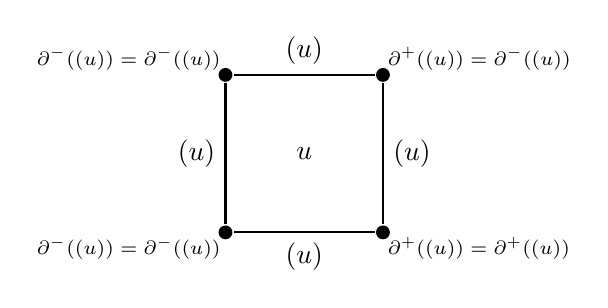
\begin{tikzpicture}[auto,scale=2,color=black,every path/.append style={thick}]
\node(UL) [fill,circle,inner sep=0pt,minimum size=5pt,label={[label distance=-.2cm]above left: 
	{\scriptsize{$\partial^- (\upperf (u)) = \partial^- (\leftf (u))$}}}] at (0,1) {};
\node(UR) [fill,circle,inner sep=0pt,minimum size=5pt,label={[label distance=-.2cm]above right: 
	{\scriptsize{$\partial^+ (\upperf (u)) = \partial^- (\rightf (u))$}}}] at (1,1) {};
\node(BL) [fill,circle,inner sep=0pt,minimum size=5pt,label={[label distance=-.2cm]below left:
	{\scriptsize{$\partial^- (\upperf (u)) = \partial^- (\leftf (u))$}}}] at (0,0) {};
\node(BR) [fill,circle,inner sep=0pt,minimum size=5pt,label={[label distance=-.2cm]below right:
	{\scriptsize{$\partial^+ (\lowerf (u)) = \partial^+ (\rightf (u))$}}}] at (1,0) {};
\draw (UL) -- (UR) node [above, midway] {$\upperf(u)$};
\draw (UR) -- (BR) node [right, midway] {$\rightf(u)$};
\draw (BR) -- (BL) node [below, midway] {$\lowerf(u)$};
\draw (BL) -- (UL) node [left, midway] {$\leftf(u)$};
\node at (0.5,0.5) {$u$};
\end{tikzpicture}
\caption{A square $u \in D_2$ and its iterated faces.}
\end{figure}

The next four equations~\ref{eq:degen-ident} tell us that for any line $f \in D_1$,
besides the identities
$\partial^\pm_1(\epsilon_1(f)) = f$ and
$\partial^\pm_2(\epsilon_2(f)) = f$ which follow from the definition of a
category, the remaining two faces of a \emph{degenerate square} are defined as
consisting of the suitable degenerate lines. Figure \ref{fig:degen-ident}
illustrates the cases of both the vertical and the horizontal category. Equation
\ref{eq:zero-unique-ident} is to make sure that in the case where we take the degenerate
square of a line which is itself degenerate and end up with a square with all four
faces degenerate, it doesn't matter if we chose the vertical or the horizontal
degeneracy but that instead we receive a unique zero-element for each $x \in D_0$.

\begin{figure} \label{fig:degen-ident} \centering
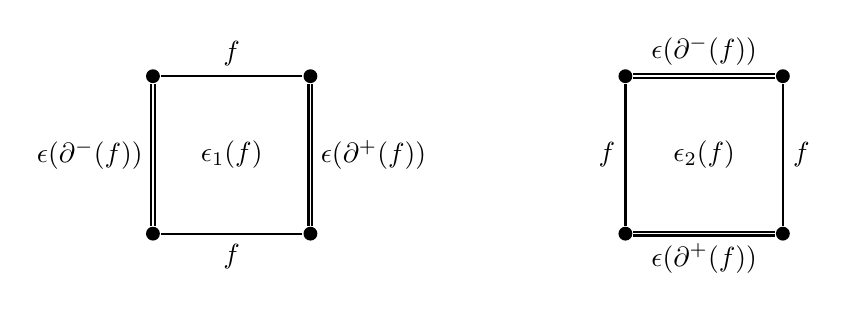
\begin{tikzpicture}[auto,scale=2,color=black,every path/.append style={thick}]
\node(UL) [fill,circle,inner sep=0pt,minimum size=5pt] at (0,1) {};
\node(UR) [fill,circle,inner sep=0pt,minimum size=5pt] at (1,1) {};
\node(BL) [fill,circle,inner sep=0pt,minimum size=5pt] at (0,0) {};
\node(BR) [fill,circle,inner sep=0pt,minimum size=5pt] at (1,0) {};
\draw (UL) -- (UR) node [above, midway] {$f$};
\draw[double] (UR) -- (BR) node [right, midway] {$\epsilon(\partial^+(f))$};
\draw (BR) -- (BL) node [below, midway] {$f$};
\draw[double] (BL) -- (UL) node [left, midway] {$\epsilon(\partial^-(f))$};
\node at (0.5,0.5) {$\epsilon_1(f)$};

\node(UL) [fill,circle,inner sep=0pt,minimum size=5pt] at (3,1) {};
\node(UR) [fill,circle,inner sep=0pt,minimum size=5pt] at (4,1) {};
\node(BL) [fill,circle,inner sep=0pt,minimum size=5pt] at (3,0) {};
\node(BR) [fill,circle,inner sep=0pt,minimum size=5pt] at (4,0) {};
\draw[double] (UL) -- (UR) node [above, midway] {$\epsilon(\partial^-(f))$};
\draw (UR) -- (BR) node [right, midway] {$f$};
\draw[double] (BR) -- (BL) node [below, midway] {$\epsilon(\partial^+(f))$};
\draw (BL) -- (UL) node [left, midway] {$f$};
\node at (3.5,0.5) {$\epsilon_2(f)$};
\end{tikzpicture}
\caption{Degenerate squares of the vertical and horizontal category for a given
line $f \in D_1$. Degenerate lines are drawn as double lines.} %%TODO "double lines"?
\end{figure}

The linearity condition~\ref{eq:linear-ident} serves to define the two faces of
a composite square that are not already fixed by the definition of vertical and
horizontal category.

\begin{figure} \label{fig:interchange} \centering
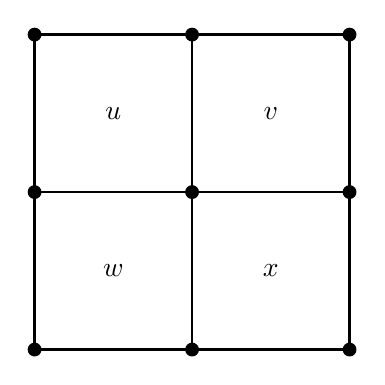
\begin{tikzpicture}[auto,scale=2,color=black,every path/.append style={thick}]
\foreach \x in {0,1,2} {
	\foreach \y in {0,1,2} {
		\node[fill,circle,inner sep=0pt,minimum size=5pt] at (\x,\y) {};
		
	}
	\draw (\x,0) -- (\x,1) -- (\x,2);
	\draw (0,\x) -- (1,\x) -- (2,\x);
}
\node at (0.5,1.5) {$u$};
\node at (1.5,1.5) {$v$};
\node at (0.5,0.5) {$w$};
\node at (1.5,0.5) {$x$};
\end{tikzpicture}
\caption{The grid we use to illustrate the composition $(x \circ_2 w) \circ_1 (v \circ_2 u)$
as well as $(x \circ_1 v) \circ_2 (w \circ_1 u)$, which are identical by the
interchange law.}
\end{figure}

The interchange law can be applied to four squares that are composable as a 
$2 \times 2$-grid to another square.
It makes sure that the result of the composition does not depend on whether we
first compose horizontally and then vertically or the other way round.
By this, it justifies to illustrate such compositions, as well as larger, iterated ones,
by ``grids'' like the one shown in figure \ref{fig:interchange}.

Starting from a given 1-skeleton it is easy to find some very simple
but nevertheless very useful and recurring examples for double categories:

\begin{example} \label{def:sq-dbl-cat}
Let $C = (C_0, C_1, \partial^-, \partial^+, \epsilon, \circ_C)$ a category. The
\textbf{square double category} on $C$ is defined by setting $D_0 \coloneqq C_0$,
$D_1 \coloneqq C_0$ and
\begin{align*}
D_2 \coloneqq \left\{ (f, g, h, i) \right| &\partial^+(f) = \partial^-(i), 
	\partial^+(i) = \partial^+(g), \\ %TODO: Make { bigger
	&\left.\partial^-(g) = \partial^+(h), 
	\partial^-(h) = \partial^-(f) \right\} \subseteq D_1^4
\end{align*}
and $\upperf$, $\lowerf$, $\leftf$, $\rightf$ to be the four projections on
this set. (To keep things consistent, I will always state the faces of a square
in the order upper, lower, left and right.) The degenerate squares are the obvious
quadruples $(f, f, \id, \id)$ and $(\id, \id, f, f)$ for a morphism $f \in C_1$.
Composing two squares $(f, g_1, h_1, i_1)$ and $(g_1, g_2, h_2, i_2)$ vertically
yields a square $(f, g_2, h_2 \circ_C h_1, i_2 \circ_C i_1)$.

Note that $f$, $g$, $h$, and $i$ do not have to form a \emph{commutative} square ---
the square double category on $C$ rather collects all possible squares in $C$.
We denote the square double category on $C$ as $\square'C$.
\end{example}

\begin{example} \label{def:comm-sq-dbl-cat}
Let again be $C = (C_0, C_1, \partial^-, \partial^+, \epsilon, \circ_C)$ a category.
We restrict the square double category on $C$ to commutative squares and receive
the \textbf{commutative square double category} on $C$:
\begin{align*}
D_0 &\coloneqq C_0 \text{,} \\
D_1 &\coloneqq C_1 \text{ and } \\
D_2 &\coloneqq \left\{ (f, g, h, i) \middle| \text{$f$, $g$, $h$, and $i$ form a
	 square and } g \circ_C h = i \circ_C f \right\} \text{.}
\end{align*}

Faces and degeneracies are trivial, for defining the the vertical composition of
two squares $(f, g_1, h_1, i_1)$ and $(g_1, g_2, h_2, i_2)$, one receives the
commutativity of the composed square by
\begin{align*}
g_2 \circ_C h_2 \circ_C h_1 &= i_2 \circ_C g_1 \circ_C h_1 \\
	&= i_2 \circ_C i_1 \circ_C f
\end{align*}
and analogously for the horizontal composition. We write $\square C$ for the
commutative square double category on $C$.
\end{example}

For the purpose of building a category of double categories we have to define what
it means for a map to preserve the structure of a double category:

\begin{defn} \label{def:dbl-functor}
A \textbf{double functor} $F$ between double categories $D$ and $E$ is a triple of maps
$(F_0, F_1, F_2)$ where $F_0 : D_0 \to E_0$, $F_1 : D_1 \to E_1$ and $F_2 : D_2
\to E_2$ such that $(F_0,F_1)$ is a functor between the 1-skeleton of $D$ and $E$
and $(F_1,F_2)$ is a functor between both the vertical and horizontal category
of $D$ and $E$. That means that all faces and degeneracies commute with with $F_1$
resp. $F_2$.
\end{defn}

\begin{lemma} \label{def:cat-of-dbl-cat}
Double functors turn the set of all double categories into a category $\DCat$.
Its initial object is the empty double category, its terminal object consists of the
double category $D$ with $D_0 = D_1 = D_2 = \{\ast\}$.
\hfill $\square$
\end{lemma}

\section{Thin structures and connections}

%TODO motivation for thin structures

\begin{defn}
Let $D$ be a double category on a category $C = (C_0, C_1)$. Then, a \textbf{thin
structure} on $D$ is a functor $T : \square C \to D$ which on the 1-skeleton is the
identity.
\end{defn}


%TODO parts of the proof? pushouts?









